\documentclass[border=4pt]{standalone}
\usepackage[T1]{fontenc}
\usepackage{lmodern}
\usepackage{amsmath}
\usepackage{pgfplots}
\pgfplotsset{compat=1.18}
\usepgfplotslibrary{groupplots,fillbetween}
\usetikzlibrary{calc,arrows.meta}
% one colour per kind of method, the same in every figure (Okabe-Ito)
\definecolor{neur}{HTML}{D55E00}   % neurons chosen by attribution
\definecolor{dirc}{HTML}{009E73}   % directions from the weird-vs-normal contrast
\definecolor{read}{HTML}{0072B2}   % readout methods and interventions chosen from readouts
\definecolor{pers}{HTML}{CC79A7}   % Assistant Axis / persona
\definecolor{ctrl}{HTML}{8C8C8C}   % random controls
\definecolor{meas}{HTML}{E69F00}   % measured outcome
\definecolor{ink}{HTML}{222222}
\pgfplotsset{
  every axis/.append style={clip=false, font=\small, axis line style={black!55}, tick style={black!55}, tick align=outside,
    label style={font=\small}, tick label style={font=\footnotesize}, title style={font=\small, align=center}},
  grid style={black!9, line width=0.4pt},
  every axis legend/.append style={font=\footnotesize, draw=none, fill=none},
  ci/.style={/pgfplots/error bars/x dir=both, /pgfplots/error bars/x explicit, /pgfplots/error bars/error bar style={line width=0.8pt}, /pgfplots/error bars/error mark=none},
  yci/.style={/pgfplots/error bars/y dir=both, /pgfplots/error bars/y explicit, /pgfplots/error bars/error bar style={line width=0.8pt}, /pgfplots/error bars/error mark=none},
}

\usepackage{CJKutf8}
\usepackage{array}
\begin{document}
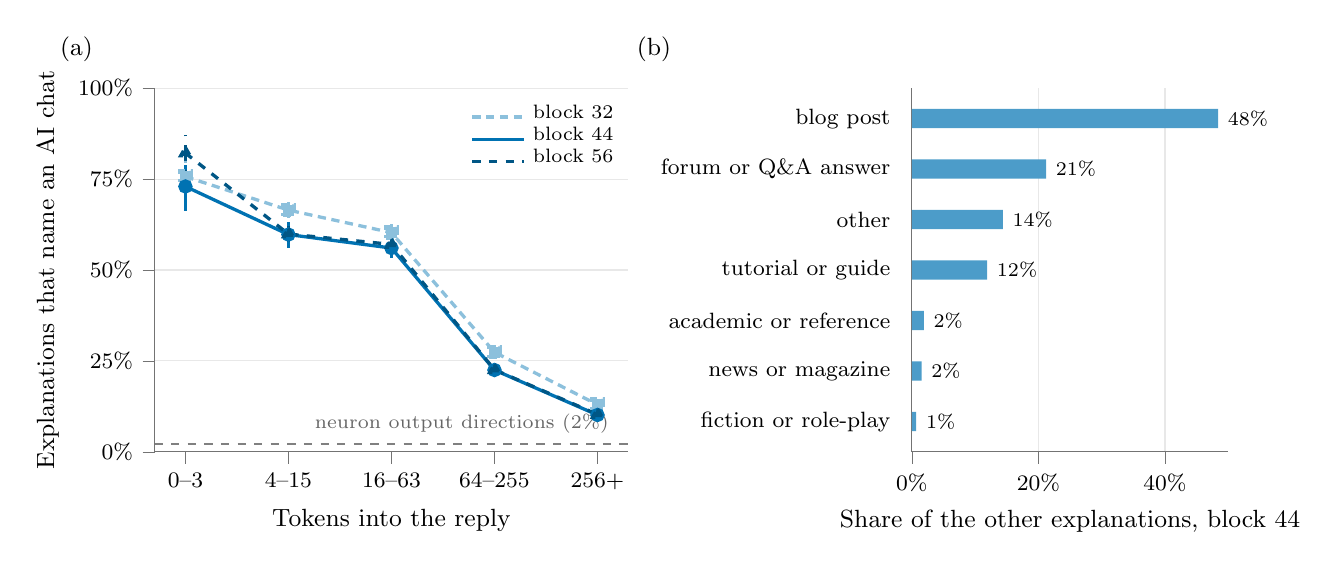
\begin{tikzpicture}
\begin{axis}[name=a, width=7.6cm, height=6.2cm, xmin=-0.3, xmax=4.3, xtick={0,1,2,3,4}, xticklabels={0--3,4--15,16--63,64--255,256+}, ymin=0, ymax=100, ytick={0,25,50,75,100}, yticklabel={$\pgfmathprintnumber{\tick}\%$}, axis x line*=bottom, axis y line*=left, ymajorgrids, xlabel={Tokens into the reply}, ylabel={Explanations that name an AI chat}, title={(a)}, title style={at={(-0.22,1.0)}, anchor=south west}]
\addplot[read!45, line width=1.2pt, mark=square*, mark size=2pt, densely dashed, yci] coordinates {(0,75.68) += (0,5.62) -= (0,6.66) (1,66.48) += (0,3.33) -= (0,3.51) (2,60.28) += (0,2.73) -= (0,2.80) (3,27.39) += (0,1.93) -= (0,1.84) (4,12.97) += (0,1.23) -= (0,1.14)};
\addplot[read, line width=1.2pt, mark=*, mark size=2pt, yci] coordinates {(0,72.97) += (0,5.88) -= (0,6.82) (1,59.75) += (0,3.50) -= (0,3.60) (2,56.04) += (0,2.78) -= (0,2.82) (3,22.50) += (0,1.81) -= (0,1.72) (4,10.14) += (0,1.11) -= (0,1.01)};
\addplot[read!75!black, line width=1.2pt, mark=triangle*, mark size=2pt, dashed, yci] coordinates {(0,82.16) += (0,4.85) -= (0,6.15) (1,59.89) += (0,3.50) -= (0,3.60) (2,57.04) += (0,2.77) -= (0,2.82) (3,22.59) += (0,1.82) -= (0,1.72) (4,10.30) += (0,1.12) -= (0,1.02)};
\node[font=\scriptsize, anchor=north east, align=left] at (axis cs:4.25,98) {\tikz\draw[read!45, line width=1.2pt, densely dashed] (0,0) -- (0.5,0); block 32\\\tikz\draw[read, line width=1.2pt] (0,0) -- (0.5,0); block 44\\\tikz\draw[read!75!black, line width=1.2pt, dashed] (0,0) -- (0.5,0); block 56};
\draw[black!50, dashed, line width=0.7pt] (axis cs:-0.3,2.28) -- (axis cs:4.3,2.28) node[pos=0.98, anchor=south east, font=\scriptsize, black!60] {neuron output directions (2\%)};
\end{axis}
\begin{axis}[at={($(a.east)+(3.6cm,0)$)}, anchor=west, width=5.6cm, height=6.2cm, xbar, bar width=7pt, xmin=0, xmax=50, ymin=-0.6, ymax=6.6, ytick={0,1,2,3,4,5,6}, yticklabels={{fiction or role-play},{news or magazine},{academic or reference},{tutorial or guide},{other},{forum or Q\&A answer},{blog post}}, y tick label style={font=\footnotesize}, major y tick style={draw=none}, xticklabel={$\pgfmathprintnumber{\tick}\%$}, axis x line*=bottom, axis y line*=left, xmajorgrids, xlabel={Share of the other explanations, block 44}, title={(b)}, title style={at={(-0.9,1.0)}, anchor=south west}, nodes near coords={\pgfmathprintnumber[fixed, precision=0]{\pgfplotspointmeta}\%}, nodes near coords style={font=\scriptsize}, point meta=x]
\addplot[fill=read!70, draw=none] coordinates {(48.39,6) (21.22,5) (14.38,4) (11.90,3) (1.88,2) (1.54,1) (0.69,0)};
\end{axis}
\end{tikzpicture}
\end{document}
